



%%%%%%%%%%%%%%%%%%%%%%%%%%%%%%%%%%%%%%%%%
% Beamer Presentation
% LaTeX Template
% Version 1.0 (10/11/12)
%
% This template has been downloaded from:
% http://www.LaTeXTemplates.com
%
% License:
% CC BY-NC-SA 3.0 (http://creativecommons.org/licenses/by-nc-sa/3.0/)
%
%%%%%%%%%%%%%%%%%%%%%%%%%%%%%%%%%%%%%%%%%

%----------------------------------------------------------------------------------------
%	PACKAGES AND THEMES
%----------------------------------------------------------------------------------------

\documentclass[aspectratio=169]{beamer}

\mode<presentation> {


% The Beamer class comes with a number of default slide themes
% which change the colors and layouts of slides. Below this is a list
% of all the themes, uncomment each in turn to see what they look like.

%\usetheme{default}
%\usetheme{AnnArbor}
%\usetheme{Antibes}
%\usetheme{Bergen}
%\usetheme{Berkeley}
%\usetheme{Berlin}
%\usetheme{Boadilla}
%\usetheme{CambridgeUS}
%\usetheme{Copenhagen}
%\usetheme{Darmstadt}
%\usetheme{Dresden}
%\usetheme{Frankfurt}
%\usetheme{Goettingen}
%\usetheme{Hannover}
%\usetheme{Ilmenau}
%\usetheme{JuanLesPins}
%\usetheme{Luebeck}
\usetheme{Madrid}
%\usetheme{Malmoe}
%\usetheme{Marburg}
%\usetheme{Montpellier}
%\usetheme{PaloAlto}
%\usetheme{Pittsburgh}
%\usetheme{Rochester}
%\usetheme{Singapore}
%\usetheme{Szeged}
%\usetheme{Warsaw}

% As well as themes, the Beamer class has a number of color themes
% for any slide theme. Uncomment each of these in turn to see how it
% changes the colors of your current slide theme.

%\usecolortheme{albatross}
%\usecolortheme{beaver}
%\usecolortheme{beetle}
%\usecolortheme{crane}
%\usecolortheme{dolphin}
%\usecolortheme{dove}
%\usecolortheme{fly}
%\usecolortheme{lily}
%\usecolortheme{orchid}
%\usecolortheme{rose}
%\usecolortheme{seagull}
%\usecolortheme{seahorse}
%\usecolortheme{whale}
%\usecolortheme{wolverine}

%\setbeamertemplate{footline} % To remove the footer line in all slides uncomment this line
%\setbeamertemplate{footline}[page number] % To replace the footer line in all slides with a simple slide count uncomment this line
\usepackage{amsmath}
\usepackage{selinput}      % Halbautomatische Auswahl der Eingabecodierung
\SelectInputMappings{      % mit Hilfe ausgewählter Glyphen
  adieresis={ä},	   % siehe: http://partners.adobe.com/public/developer/en/opentype/glyphlist.txt
  germandbls={ß},
  Euro={€}
}

\definecolor{UOSred}{rgb}{0.6745098039215686, 0.02352241176470588, 0.2039215686274510} % UBC Blue (primary)
\definecolor{UOSgrey}{rgb}{0.8117647058823522, 0.8117647058823522, 0.8117647058823522} % UBC Grey (secondary)

\setbeamercolor{palette primary}{bg=UOSred,fg=white}
\setbeamercolor{palette secondary}{bg=UOSred,fg=white}
\setbeamercolor{palette tertiary}{bg=UOSred,fg=white}
\setbeamercolor{palette quaternary}{bg=UOSred,fg=white}
\setbeamercolor{structure}{fg=UOSred} % itemize, enumerate, etc
\setbeamercolor{section in toc}{fg=UOSred} % TOC sections

%gets rid of bottom navigation bars
\setbeamertemplate{footline}[frame number]{}

%gets rid of bottom navigation symbols
\setbeamertemplate{navigation symbols}{}

\addtobeamertemplate{footline}{%
  \leavevmode%
  \hbox{%
  \begin{beamercolorbox}[wd=\paperwidth,ht=2.25ex,dp=1ex,center]{author in head/foot}%
     \insertsectionnavigationhorizontal{\paperwidth}{}{}
  \end{beamercolorbox}}%

}

% Override palette coloring with secondary
\setbeamercolor{subsection in head/foot}{bg=UOSgrey,fg=white}

%\setbeamertemplate{navigation symbols}{} % To remove the navigation symbols from the bottom of all slides uncomment this line
}
\usepackage{hyperref}
\usepackage{graphicx} % Allows including images
\usepackage{grffile}
\usepackage{booktabs} % Allows the use of \toprule, \midrule and \bottomrule in tables
\graphicspath{{images/}}
%----------------------------------------------------------------------------------------
%	TITLE PAGE
%----------------------------------------------------------------------------------------

\title[Aufgabe 4.3]{Aufgabe 4.3} % The short title appears at the bottom of every slide, the full title is only on the title page

\author{T. Adam, M. ben Ahmed} % Your name
\institute[UOS] % Your institution as it will appear on the bottom of every slide, may be shorthand to save space
{

Universität Osnabrück \\ % Your institution for the title page

\medskip
\textit{Æ} % Your email address


}
\date{\today} % Date, can be changed to a custom date

\begin{document}

\begin{frame}
\titlepage % Print the title page as the first slide
\end{frame}


%----------------------------------------------------------------------------------------
%	PRESENTATION SLIDES
%----------------------------------------------------------------------------------------


%------------------------------------------------



\begin{frame}
	\frametitle{Aufgabe 4.3 - KCT Heuristiken}
	\begin{columns}[c] % The "c" option specifies centered vertical alignment while the "t" option is used for top vertical alignment
		
		\column{.8\textwidth} % Left column and width
		\textbf{Heuristics for the K-Cardinality Tree and Subgraph Problems (1997)}
		\begin{itemize}
			\item M. Ehrgott, J. Freitag, H. W. Hamacher, F. Maffiali $\dagger$
			\item 3 Klassen von Heuristiken für EKCT
			\item 2 Klassen von Heuristiken für NKCT
			\item Umwandlung von NKCT $\Rightarrow$ EKCT
		\end{itemize}	
	\end{columns}
	\end{frame}
	
%------------------------------------------------


\begin{frame}
	\frametitle{Greedy Klasse}
	\begin{columns}[c] % The "c" option specifies centered vertical alignment while the "t" option is used for top vertical alignment
		
		\column{.55\textwidth} % Left column and width
		\textbf{MST basierte Heuristiken}
		\begin{itemize}
			\item Prim mit $|E(mst)| = k$
			\item Kruskal mit mehreren Zusammenhangskomp.
			\item Kruskal mit einer Zusammenhangskomp.
		\end{itemize}
		\column{.25\textwidth} % Right column and width
		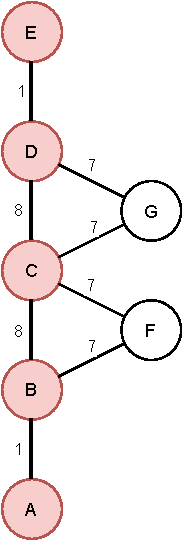
\includegraphics[scale=.6]{greedy_optimal.pdf}
		k = 4\\
		$c^* = 18$
		
		
	\end{columns}
	\end{frame}
	
%------------------------------------------------

\begin{frame}
	\frametitle{Greedy - k-CardPrim}
	\begin{columns}[c] % The "c" option specifies centered vertical alignment while the "t" option is used for top vertical alignment
		
		\column{.55\textwidth} % Left column and width
		\textbf{k-CardPrim}
		\begin{itemize}
			\item Starte Alg. von Prim für alle Knoten
			\item Breche ab, sobald MST $k+1$ Knoten enthält
			\item Gebe günstigsten MST zurück
		\end{itemize}
		\column{.25\textwidth} % Right column and width
		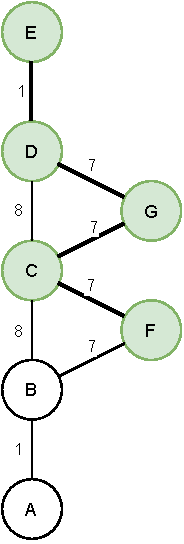
\includegraphics[scale=.6]{greedy_prim1.pdf}
		k = 4\\
		$c = 22$
		
		
	\end{columns}
	\end{frame}
	
%------------------------------------------------


\begin{frame}
	\frametitle{Greedy - DualGreedy1}
	\begin{columns}[c] % The "c" option specifies centered vertical alignment while the "t" option is used for top vertical alignment
		
		\column{.55\textwidth} % Left column and width
		\textbf{DualGreedy1}
		\begin{itemize}
			\item Starte mit Ausgangsgraph
			\item Lösche teuerste Kante
			\item Wiederhole, solange min. eine Zhk. mit min. $k+1$ Knoten existiert 
		\end{itemize}
		\column{.25\textwidth} % Right column and width
		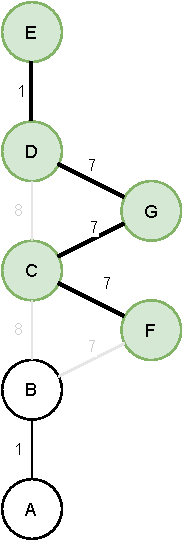
\includegraphics[scale=.6]{greedy_greedy1.pdf}
		k = 4\\
		$c = 22$
		
		
	\end{columns}
	\end{frame}
	
%------------------------------------------------



\begin{frame}
	\frametitle{Greedy - DualGreedy2}
	\begin{columns}[c] % The "c" option specifies centered vertical alignment while the "t" option is used for top vertical alignment
		
		\column{.55\textwidth} % Left column and width
		\textbf{DualGreedy2}
		\begin{itemize}
			\item Starte mit Ausgangsgraph
			\item Lösche teuerste Kante inkl. Knoten, deren Löschung keine weiteren Zhk. erzeugt
			\item Wiederhole, bis $k+1$ Knoten im Graph bleiben 
		\end{itemize}
		\column{.25\textwidth} % Right column and width
		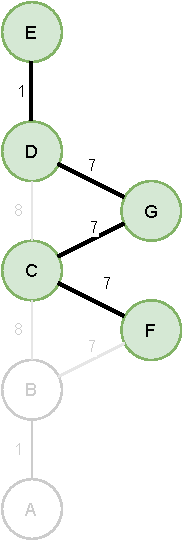
\includegraphics[scale=.6]{greedy_greedy2.pdf}
		k = 4\\
		$c = 22$
		
		
	\end{columns}
	\end{frame}
	
%------------------------------------------------

\begin{frame}
	\frametitle{Path Klasse}
	\begin{columns}[c] % The "c" option specifies centered vertical alignment while the "t" option is used for top vertical alignment
		
		\column{.55\textwidth} % Left column and width
		\textbf{Shortest-Path basierte Heuristiken}
		\begin{itemize}
			\item Dijkstra mit max. Pfadlänge $k$ (Gewichte)
			\item Dijkstra mit max. Pfadlänge $k$ (Kardinalität)
			\item Erweitere Pfade aus Dijkstra $<k$ mit Prim
			\item Führe beide Dijkstra Alg. aus und wähle beste Lösung
		\end{itemize}
		\column{.25\textwidth} % Right column and width
		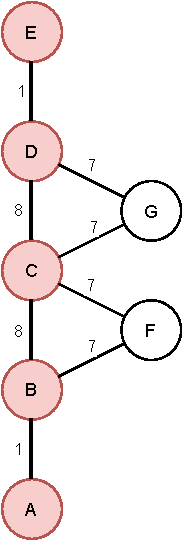
\includegraphics[scale=.6]{path_optimal.pdf}
		k = 4\\
		$c^* = 18$
		
		
	\end{columns}
	\end{frame}
	
%------------------------------------------------


\begin{frame}
	\frametitle{Path - k-DijkstraA(B)}
	\begin{columns}[c] % The "c" option specifies centered vertical alignment while the "t" option is used for top vertical alignment
		
		\column{.55\textwidth} % Left column and width
		\textbf{k-DijkstraA(B)}
		\begin{itemize}
			\item Dijkstra mit max. Pfadlänge $k$ von Knoten $s \Rightarrow x$
			\item Führe zusätzlich \texttt{len[]} und \texttt{dist[]} ein
			\item Speichere Länge und Gewicht des bisher besten Pfades
			\item (A) \texttt{dist[x]} wird aktualisiert, wenn Gesamtgewicht echt kleiner wird
			\item (B) \texttt{dist[x]} wird aktualisiert, wenn Gesamtgewicht kleiner oder Länge größer wird
			\item Füge Knoten mit minimalen \texttt{dist[]} am Ende des Pfades hinzu solange $<k$ Kanten
		\end{itemize}
		\column{.25\textwidth} % Right column and width
		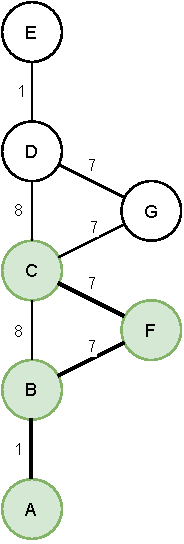
\includegraphics[scale=.6]{path_dijkstraAB.pdf}
		k = 4\\
		
		
	\end{columns}
	\end{frame}
	
%------------------------------------------------


\begin{frame}
	\frametitle{Path - DijkstraPrim-A(B)}
	\begin{columns}[c] % The "c" option specifies centered vertical alignment while the "t" option is used for top vertical alignment
		
		\column{.55\textwidth} % Left column and width
		\textbf{DijkstraPrim-A(B)}
		\begin{itemize}
			\item Wende k-DijkstraA(B) für alle Knoten an
			\item Erweitere Pfade kürzer als $k$ mit Prim
			\item Wähle beste Lösung
		\end{itemize}
		\column{.25\textwidth} % Right column and width
		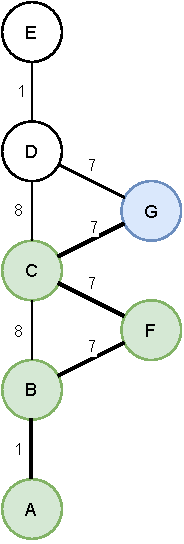
\includegraphics[scale=.6]{path_dijkstraAprim.pdf}
		k = 4\\
		$c = 22$
		
		
	\end{columns}
	\end{frame}
	
%------------------------------------------------


\begin{frame}
	\frametitle{Path - DijkstraPrim}
	\begin{columns}[c] % The "c" option specifies centered vertical alignment while the "t" option is used for top vertical alignment
		
		\column{.55\textwidth} % Left column and width
		\textbf{DijkstraPrim}
		\begin{itemize}
			\item Führe DijkstraPrim-A aus
			\item Führe DijkstraPrim-B aus
			\item Wähle beste Lösung 
		\end{itemize}
		\column{.25\textwidth} % Right column and width
		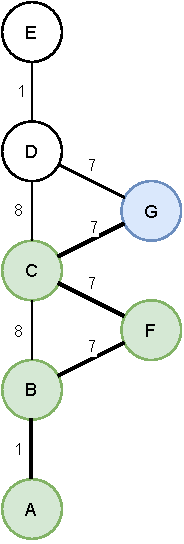
\includegraphics[scale=.6]{path_dijkstraAprim.pdf}
		k = 4\\
		$c = 22$
		
		
	\end{columns}
	\end{frame}
	
%------------------------------------------------

\begin{frame}
	\frametitle{DynamicTree Klasse}
	\begin{columns}[c] % The "c" option specifies centered vertical alignment while the "t" option is used for top vertical alignment
		
		\column{.55\textwidth} % Left column and width
		\textbf{Dynamic Programming basierte Heuristiken}
		\begin{itemize}
			\item DynamicTree findet garantiert einen optimalen KCT in gegebenen MST
			\item Erzeuge MST mit Prim und wende DT an
			\item Erzeuge MST mit 
			\item Führe beide Dijkstra Alg. aus und wähle beste Lösung
		\end{itemize}
		\column{.25\textwidth} % Right column and width
		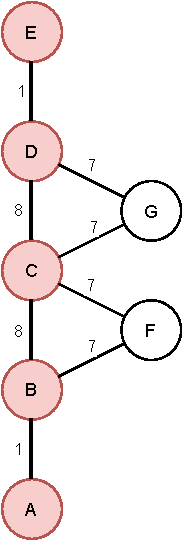
\includegraphics[scale=.6]{path_optimal.pdf}
		k = 4\\
		$c^* = 18$
		
		
	\end{columns}
	\end{frame}
	
%------------------------------------------------

\begin{frame}
	\frametitle{DynamicTree - DynamicTreePrim}
	\begin{columns}[c] % The "c" option specifies centered vertical alignment while the "t" option is used for top vertical alignment
		
		\column{.55\textwidth} % Left column and width
		\textbf{DynamicTreePrim}
		\begin{itemize}
			\item Finde MST mit Prim
			\item Führe Dynmic Tree auf MST aus
		\end{itemize}
		\column{.25\textwidth} % Right column and width
		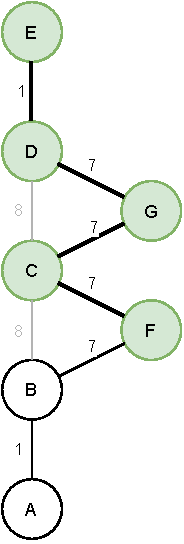
\includegraphics[scale=.6]{dynamic_prim.pdf}
		k = 4\\
		$c = 22$
		
		
	\end{columns}
	\end{frame}
	
%------------------------------------------------


\begin{frame}
	\frametitle{DynamicTree - DynamicDijkstraPath}
	\begin{columns}[c] % The "c" option specifies centered vertical alignment while the "t" option is used for top vertical alignment
		
		\column{.55\textwidth} % Left column and width
		\textbf{DynamicDijkstraPath}
		\begin{itemize}
			\item Führe DijkstraPrim aus
			\item Erweitere Ergebnis mit Prim zu MST
			\item Führe Dynamic Tree auf MST aus
		\end{itemize}
		\column{.25\textwidth} % Right column and width
		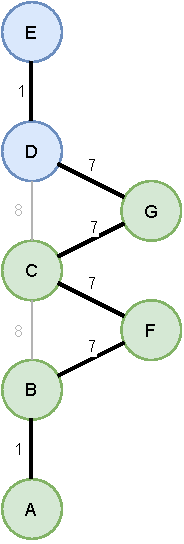
\includegraphics[scale=.6]{dynamic_dijkstra.pdf}
		k = 4\\
		$c = 22$
		
		
	\end{columns}
	\end{frame}
	
%------------------------------------------------

\begin{frame}
	\frametitle{DynamicTree - DynamicDijkstraTree}
	\begin{columns}[c] % The "c" option specifies centered vertical alignment while the "t" option is used for top vertical alignment
		
		\column{.55\textwidth} % Left column and width
		\textbf{DynamicDijkstraTree}
		\begin{itemize}
			\item Führe k-Dijkstra-A(B) aus
			\item Erweitere Pfade mit Prim zu MSTs
			\item Führe Dynamic Tree auf MSTs aus
		\end{itemize}
		\column{.25\textwidth} % Right column and width
		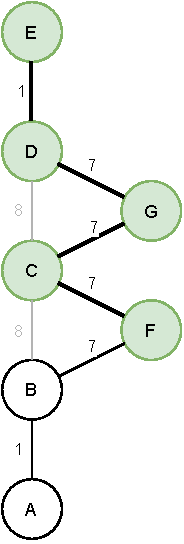
\includegraphics[scale=.6]{dynamic_prim.pdf}
		k = 4\\
		$c = 22$
		
		
	\end{columns}
	\end{frame}
%------------------------------------------------
\begin{frame}
\frametitle{NKCT $\rightarrow$ EKCT}
\begin{columns}[c] % The "c" option specifies centered vertical alignment while the "t" option is used for top vertical alignment
	
	\column{.45\textwidth} % Left column and width
	\textbf{NKCT(G) $\rightarrow$ EKCT(G')}
	\begin{itemize}
		\item Verdoppele alle Knoten in $G$
		\item Kantengewicht zwischen verdoppelten Knoten entspricht Knotengewicht
		\item Sonstige Kantengewichte: $(|E|+1)\cdot w_{max}$
		\item EKCT mit $k' = 2k + 1$ auf $G'$ anwenden
	\end{itemize}
	\column{.45\textwidth} % Right column and width
	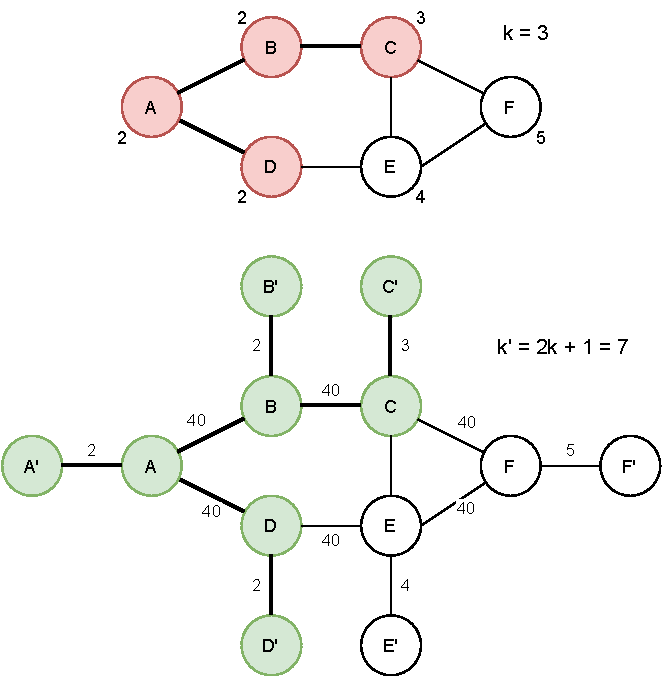
\includegraphics[scale=.6]{nekctk.pdf}
	
	
\end{columns}
\end{frame}
%------------------------------------------------
\begin{frame}
	\frametitle{Tests}
	\begin{columns}[c] % The "c" option specifies centered vertical alignment while the "t" option is used for top vertical alignment
		
		\column{.95\textwidth} % Left column and width
		\textbf{Laufzeiten und Instanzen}
		\begin{itemize}
			\item Komplexität der Algorithmen in  $\mathcal{O}(n^3)$
			\item Außer DynamicTree und DualGreedy in $\mathcal{O}(n^4)$
			\item Alle Instanzen lösbar innerhalb von Sekunden
			\item 20 Random Graphen mit jeweils $[10,20,30]$ Knoten
			\item Zufällige generierte Kantengewichte (exponenziell-, gleich- und normalverteilt) 
			\item Getestete k: $3 \leq k \leq n-2$
			\item Relativ große $k$ realistischer als kleine $k$: Ölfeld Bsp. $k= \frac{n}{2}$
		\end{itemize}
		
		
		
	\end{columns}
	\end{frame}
	%------------------------------------------------

\begin{frame}
	\frametitle{Ergebnisse}
	
	\begin{columns}[c] % The "c" option specifies centered vertical alignment while the "t" option is used for top vertical alignment
		
		\column{.4\textwidth} % Left column and width
		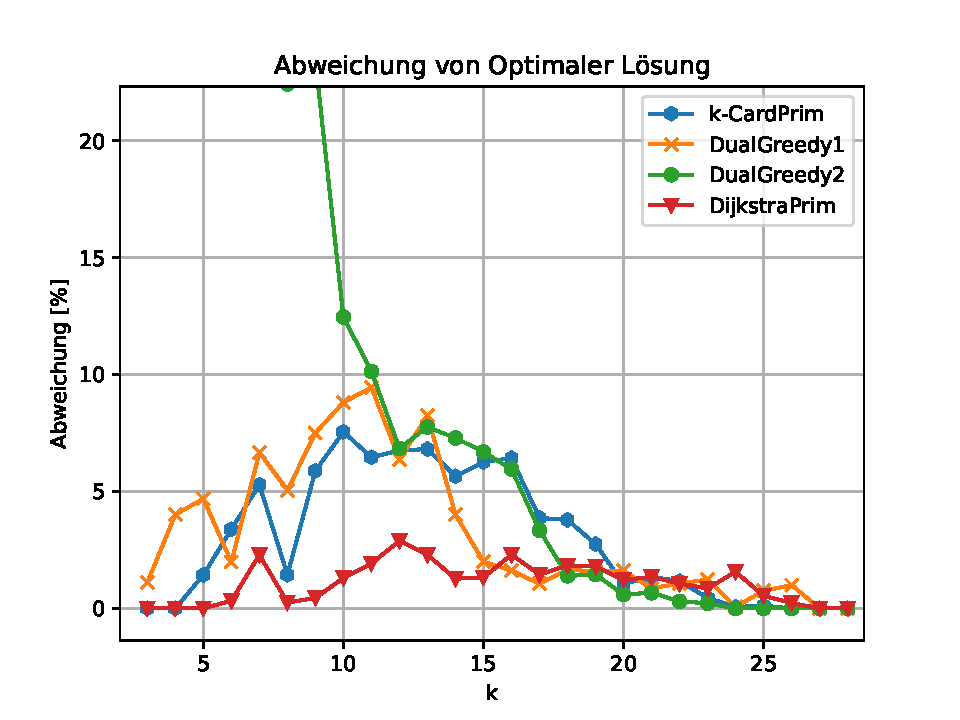
\includegraphics[scale=.45]{plot_greedy-path.pdf}
		\column{.55\textwidth} % Right column and width
		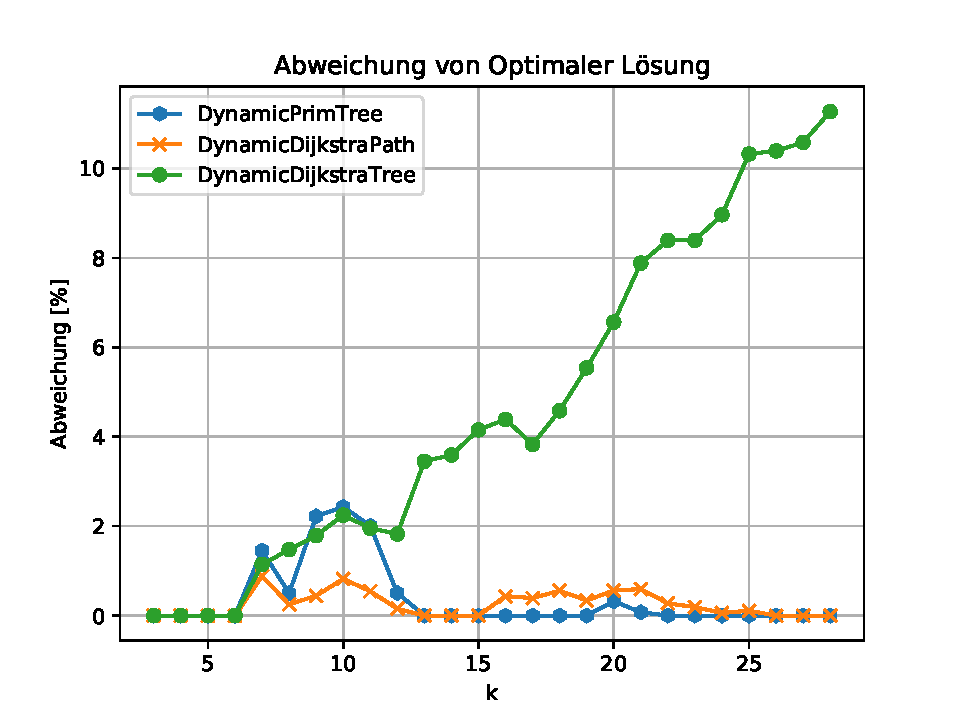
\includegraphics[scale=.45]{plot_dynamic.pdf}
		
		
	\end{columns}
	\centering
	Genereller Graph mit 30 Knoten
	\end{frame}
	
%------------------------------------------------


\end{document} 